\section{Agregar Auxiliar}

Un paciente podrá ingresar los datos de un nuevo Auxiliar el cual
estará a cargo de un tratamiento médico del paciente.

\subsubsection{Procedimiento}
\begin{enumerate}
	
	\item Da clic en el icono \textbf{Auxiliares} de la pantalla \textbf{Menú Principal}.

		\begin{figure}[!htbp]			\hypertarget{fig:mpPaciente6}{\hspace{1pt}}
		\begin{center}
			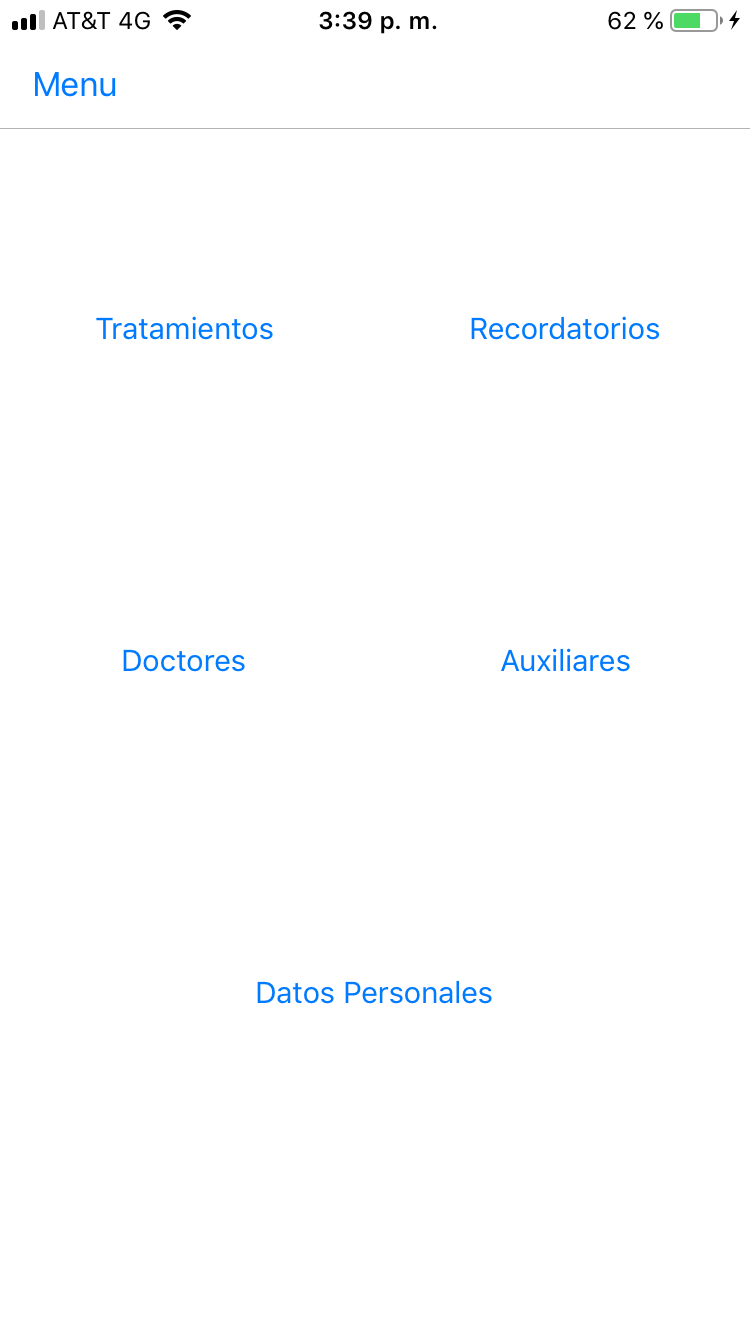
\includegraphics[height=0.4\textheight]{Paciente/AgregarAuxiliar/images/mpPaciente}
			\caption{Menú Principal Paciente}
			\label{fig:mpPaciente6}
		\end{center}
	\end{figure}

	\item Se mostrará la pantalla \textbf{Auxiliares}. 
	\newpage
	\begin{figure}[!htbp]			
		\hypertarget{fig:Auxiliares}{\hspace{1pt}}
		\begin{center}
			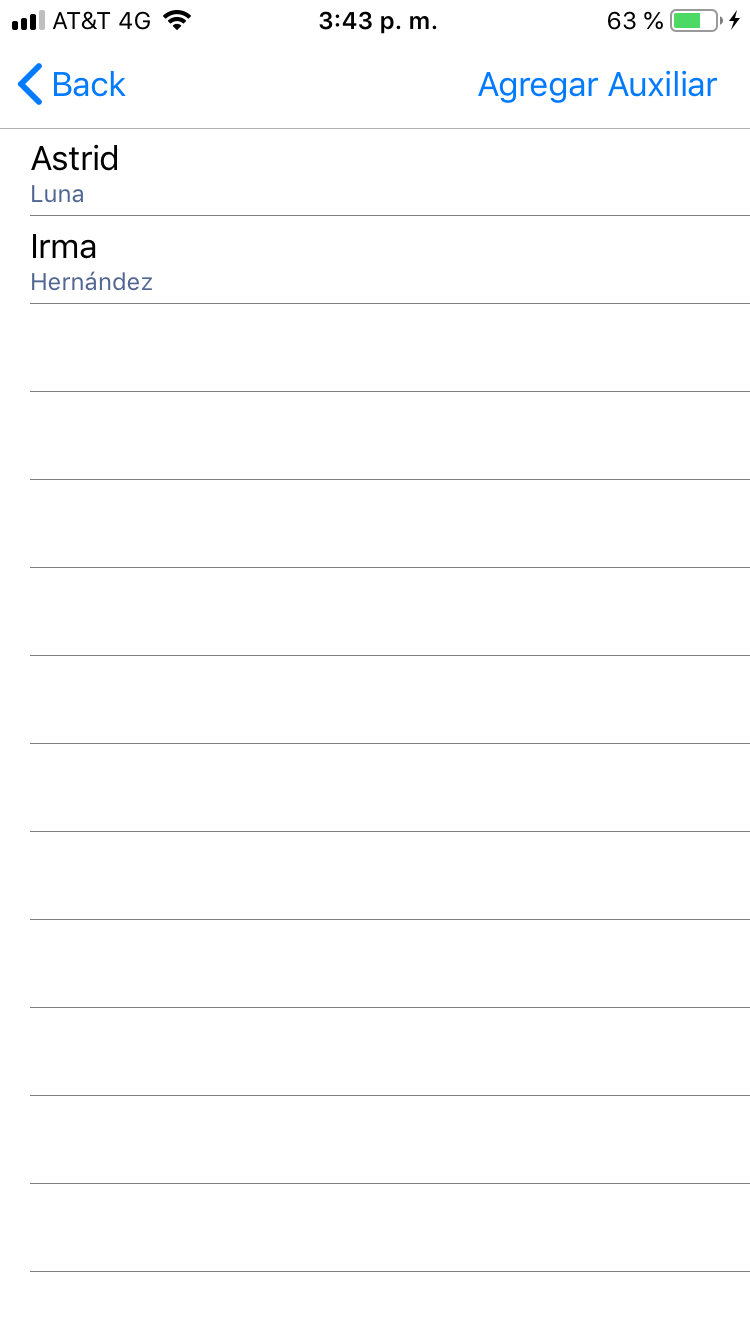
\includegraphics[height=0.4\textheight]{Paciente/AgregarAuxiliar/images/Auxiliares}
			\caption{Auxiliares}
			\label{fig:Auxiliares}
		\end{center}
	\end{figure}

	\item Da clic en el botón \textbf{Agregar Auxiliar} de la pantalla \textbf{Auxiliares}.
	
	\item Se mostrará la pantalla \textbf{Agregar Auxiliar}.
	
	\begin{figure}[!htbp]			
		\hypertarget{fig:AgregarAuxiliar}{\hspace{1pt}}
		\begin{center}
			
\includegraphics[height=0.4\textheight]{Paciente/AgregarAuxiliar/images/AgregarAuxiliar}
			\caption{Agregar Auxiliar}
			\label{fig:AgregarAuxiliar}
		\end{center}
	\end{figure}

	\begin{figure}[!htbp]			
		\hypertarget{fig:AgregarAuxiliar2}{\hspace{1pt}}
		\begin{center}
			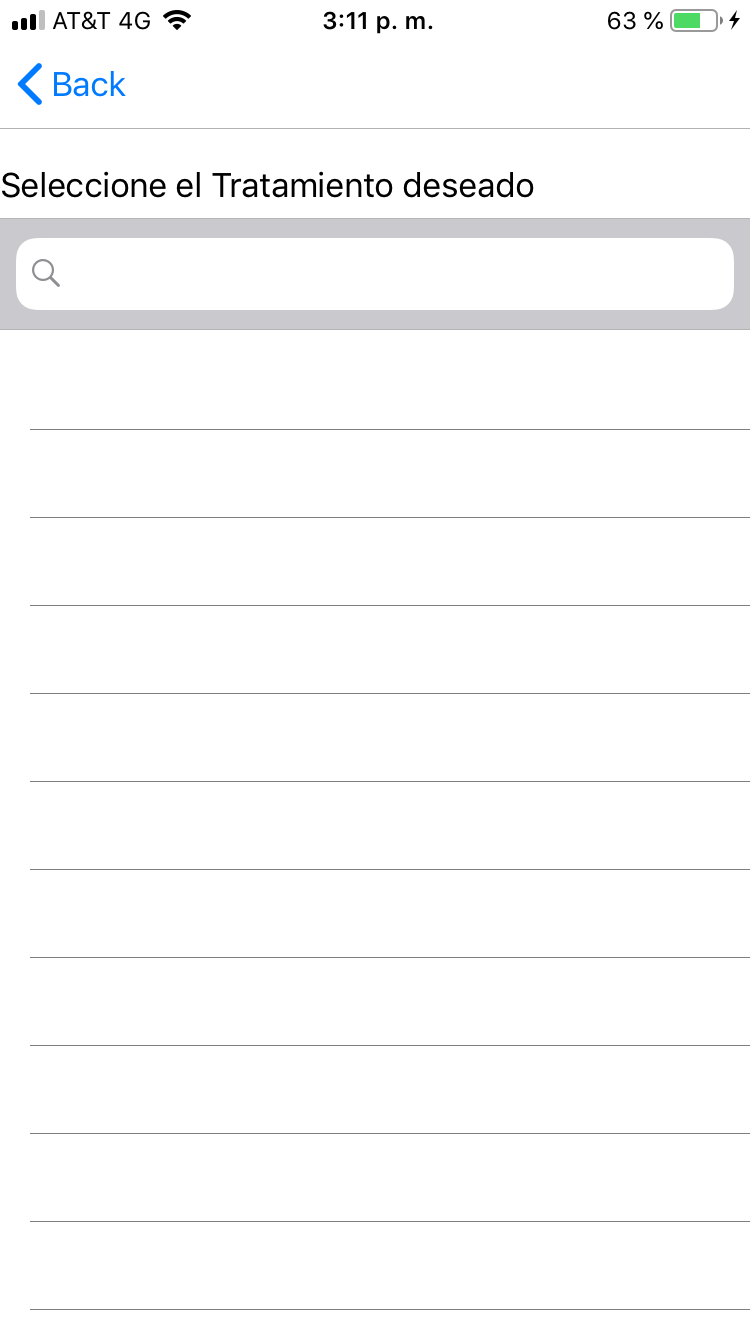
\includegraphics[height=0.4\textheight]{Paciente/AgregarAuxiliar/images/AgregarAuxiliar2}
			\caption{Agregar Auxiliar}
			\label{fig:AgregarAuxiliar2}
		\end{center}
	\end{figure}

	\item Ingrese el auxiliar deseado y el tratamiento al que estará asociado ese auxiliar en la pantalla \textbf{Agregar Tratamiento}.
	
	\item Da clic en el botón Agregar Auxiliar.
	
\end{enumerate}

